% !TeX program = xelatex
% !TeX encoding = UTF-8
% !TeX TXS-program:compile = txs:///xelatex | txs:///xelatex
\documentclass[aspectratio=169, table, 12pt]{beamer}

% Preamble bersama seluruh slide mata kuliah ini.
% Dipanggil dari slides/sessionXX/sessionXX.tex tepat sesudah baris
% \documentclass[aspectratio=169, table, 12pt]{beamer}
% Paket tambahan yang hanya dibutuhkan satu sesi ditulis di berkas sesi itu.

\usepackage{colortbl}
\usepackage{xcolor}
\usepackage{listings}
\usepackage{tabularx}
\usepackage{booktabs}
\usepackage{tikz}
\usepackage{pgfplots}
\usepackage{fontspec}
\usepackage[english,bahasai]{babel}
\pgfplotsset{compat=1.18}
\usetikzlibrary{arrows.meta, positioning, calc, fit, shapes.geometric,
  shapes.multipart, backgrounds, matrix, chains, trees}

\makeatletter
\def\input@path{{../theme/}}
\makeatother
\graphicspath{{../theme/}{../../figures/}}
% Stub symlink Windows memakai tema cadangan sampai aset institusi tersedia.
\IfFileExists{../theme/beamerthemePradita.sty}{%
  \usetheme{Pradita}
}{%
  \usetheme{Madrid}
  \setmainfont{TeX Gyre Heros}
  \setsansfont{TeX Gyre Heros}
  \setbeamertemplate{navigation symbols}{}
}

\definecolor{praditagreen}{RGB}{37, 113, 71}
\setbeamercolor{structure}{fg=praditagreen}
\setbeamercolor{palette primary}{bg=praditagreen,fg=white}
\setbeamercolor{palette secondary}{bg=praditagreen!80!black,fg=white}
\setbeamercolor{palette tertiary}{bg=praditagreen!60!black,fg=white}
\setbeamerfont{frametitle}{size=\large}
\setbeamertemplate{caption}[numbered]

% Ukuran header mengikuti teks agar judul panjang tidak menabrak logo.
\setbeamercolor{frametitle}{bg=white,fg=black}
\setbeamertemplate{frametitle}{%
  \begin{beamercolorbox}[wd=\paperwidth,sep=0.2cm]{frametitle}
    \begin{minipage}[c]{0.77\paperwidth}
      \raggedright\fontsize{16}{18}\selectfont\bfseries\insertframetitle
      \ifx\insertframesubtitle\empty\else
        \par\small\mdseries\insertframesubtitle
      \fi
    \end{minipage}\hfill
    \begin{minipage}[c]{0.15\paperwidth}
      \IfFileExists{../theme/classFiles/logo_universitas.png}{%
        
\includegraphics[width=\linewidth]{../theme/classFiles/logo_universitas.png}%
      }{}
    \end{minipage}
  \end{beamercolorbox}
}
\setbeamertemplate{footline}{%
  \ifnum\value{framenumber}>1
    \begin{beamercolorbox}[wd=\paperwidth,ht=0.35cm,dp=0.15cm,
      leftskip=0.3cm,rightskip=0.3cm]{palette primary}
      \footnotesize\bfseries\insertframenumber/\inserttotalframenumber
      \hfill IT40813
    \end{beamercolorbox}
  \fi
}
\DeclareRobustCommand{\berkas}[1]{\path{#1}}

% Tema membuat garis tabel berwarna putih. Dikembalikan agar tabel terbaca.
\arrayrulecolor{black}
\setlength{\arrayrulewidth}{0.5pt}

\lstdefinelanguage{yaml}{
  basicstyle=\ttfamily\scriptsize,
  keywordstyle=\color{blue}\bfseries,
  commentstyle=\color{gray}\itshape,
  stringstyle=\color{red},
  showstringspaces=false,
  breaklines=true,
  frame=lines,
  numbers=none,
  backgroundcolor=\color{lightgray!10},
  tabsize=2,
  morecomment=[l]{\#}
}

\lstdefinelanguage{json}{
  basicstyle=\ttfamily\scriptsize,
  stringstyle=\color{red},
  commentstyle=\color{gray},
  breaklines=true,
  showstringspaces=false,
  tabsize=2,
  numbers=none,
  frame=lines,
  backgroundcolor=\color{lightgray!10},
  string=[s]{"}{"}
}

\lstdefinelanguage{bash}{
  keywords={},
  basicstyle=\ttfamily\scriptsize,
  ndkeywords={docker, kubectl, helm, curl, git, terraform},
  ndkeywordstyle=\color{purple}\bfseries,
  sensitive=true,
  commentstyle=\color{gray},
  numbers=none,
  breaklines=true,
  frame=lines,
  backgroundcolor=\color{lightgray!10},
  tabsize=2,
  comment=[l]{\#},
  showstringspaces=false
}

\lstdefinelanguage{http}{
  keywords={GET, POST, PUT, PATCH, DELETE, HEAD, OPTIONS, HTTP},
  basicstyle=\ttfamily\scriptsize,
  keywordstyle=\color{blue}\bfseries,
  sensitive=true,
  numbers=none,
  breaklines=true,
  frame=lines,
  backgroundcolor=\color{lightgray!10},
  tabsize=2,
  showstringspaces=false
}

\subtitle{IT40813 · IT Governance, Risk \& Compliance}
\author{\textbf{Alfa Yohannis}}


% Sampul membatasi judul di panel putih tema rujukan Pradita.
\setbeamertemplate{title page}{%
  \begin{tikzpicture}[remember picture,overlay]
    \node[anchor=north west,inner sep=0pt,text width=8.8cm]
      at ([xshift=1cm,yshift=-3.15cm]current page.north west) {%
        {\small\insertsubtitle\par}\vspace{0.25cm}
        \resizebox{8.8cm}{!}{\begin{minipage}{12cm}
          \raggedright\color{praditagreen}\bfseries\inserttitle
        \end{minipage}}
      };
    \node[anchor=south west,inner sep=0pt]
      at ([xshift=1cm,yshift=1.65cm]current page.south west)
      {\small\insertdate};
    \node[anchor=west,inner sep=0pt,text=white]
      at ([xshift=0.8cm,yshift=0.75cm]current page.south west)
      {\small\insertauthor};
  \end{tikzpicture}
}


\title{\Huge Merancang Sistem\\ \vspace{10pt} Tata Kelola Target}
\date{Pertemuan 08}

\begin{document}

\frame{\titlepage}

\begin{frame}
  \frametitle{Isi Pertemuan}
  \vspace{14pt}
  \begin{columns}[t]
    \column{0.5\textwidth}
    {\small\tableofcontents[sections={1-4}]}

    \column{0.5\textwidth}
    {\small\tableofcontents[sections={5-8}]}
  \end{columns}
\end{frame}

\begin{frame}{\hfill}
  \centering
  \Huge{\textbf{Semua setuju arah transformasi.\\Siapa menyetujui apa?}}
\end{frame}

\section{Tujuan dan Konteks}

\begin{frame}{{\Large Tujuan Pembelajaran}}
  \vspace{10pt}
  \begin{itemize}
    \item Merancang struktur tata kelola target, termasuk forum keputusan, peran kunci, dan matriks
          RACI.
    \item Menetapkan target kapabilitas COBIT dan profil target NIST CSF yang selaras dengan
          \textit{risk appetite}.
    \item Mengaitkan praktik ITIL 4 dengan objektif manajemen COBIT untuk menjalankan layanan TI
          sehari-hari.
  \end{itemize}
\end{frame}

\begin{frame}{{\Large Masalah: Semua Setuju, Keputusan Tidak Jelas}}
  \vspace{6pt}
  \small
  \begin{itemize}
    \item Misalkan mitra asuransi meminta integrasi untuk 6.000 klaim per bulan.
    \item Tim platform ingin membuka data, pemilik layanan khawatir, hukum meminta pembatasan
          tujuan.
    \item Usulan berpindah antarforum selama 4 bulan, sehingga 24.000 klaim tetap manual.
    \item Dua pertanyaan: siapa menyetujui pembukaan data, dan siapa memegang akuntabilitas rekam
          medis terpadu?
    \item Hasil kerja: model tata kelola target untuk tonggak C3.
  \end{itemize}
\end{frame}

\begin{frame}{{\Large Diagram Konsep Bab 8}}
  \centering
  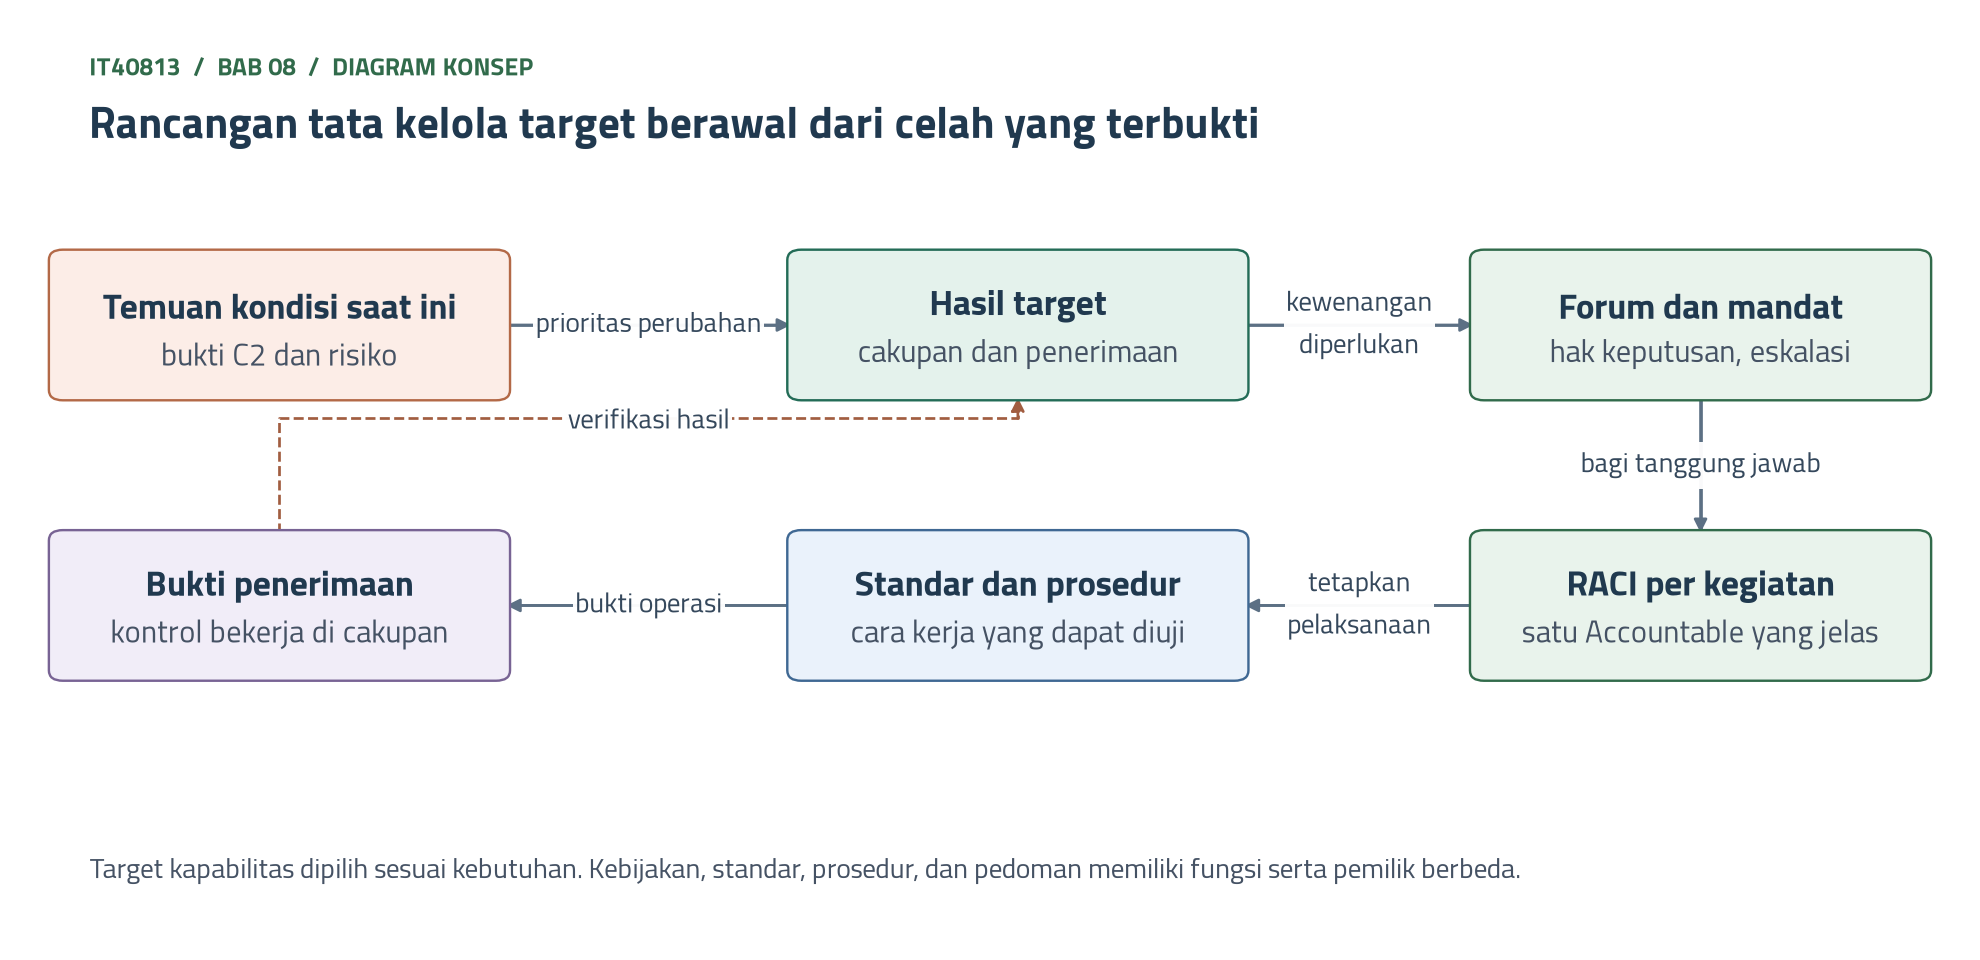
\includegraphics[width=0.96\textwidth,height=0.77\textheight,keepaspectratio]{../../figures/ch08-diagram-konsep.png}
  \label{fig:session08-ilustrasi-bab}
\end{frame}

\section{Dari Celah ke Target}

\begin{frame}{{\Large Empat Tahap Panduan Desain}}
  \vspace{4pt}
  \begin{center}
    \resizebox{0.92\textwidth}{!}{\begin{tikzpicture}[
  font=\scriptsize,
  tahap/.style={draw, rounded corners, align=center, text width=2.4cm,
    minimum height=1.05cm, fill=blue!8},
  capstone/.style={draw, rounded corners, align=center, minimum height=1.2cm},
  panah/.style={-{Stealth[length=2mm]}, thick},
  tautan/.style={dashed, -{Stealth[length=2mm]}}]
  \node[anchor=south west, font=\scriptsize\bfseries] at (-1.3,0.55)
    {Panduan desain COBIT 2019};
  \node[tahap] (t1) at (0,0) {1. Konteks\\dan strategi};
  \node[tahap] (t2) at (3,0) {2. Cakupan awal};
  \node[tahap] (t3) at (6,0) {3. Penyempurnaan\\cakupan};
  \node[tahap, fill=orange!12] (t4) at (9,0) {4. Kesimpulan\\rancangan};
  \draw[panah] (t1) -- (t2);
  \draw[panah] (t2) -- (t3);
  \draw[panah] (t3) -- (t4);
  \node[anchor=south west, font=\scriptsize\bfseries] at (0.15,-1.3) {Capstone Medikara};
  \node[capstone, fill=blue!8, text width=2.4cm] (c1) at (0,-2.2)
    {C1: strategi,\\hak keputusan,\\kewajiban};
  \node[capstone, fill=blue!8, text width=5.4cm] (c2) at (4.5,-2.2)
    {C2: Bab 4 memilih 6 objektif awal;\\Bab 5 sampai 7: risiko dan 13 celah};
  \node[capstone, fill=green!10, text width=2.4cm] (c3) at (9,-2.2)
    {C3: target, forum,\\RACI, kebijakan};
  \draw[tautan] (t1.south) -- (c1.north);
  \draw[tautan] (t2.south) -- (t2.south |- c2.north);
  \draw[tautan] (t3.south) -- (t3.south |- c2.north);
  \draw[tautan] (t4.south) -- (c3.north);
\end{tikzpicture}
}
  \end{center}
  \small Bab 4 memilih enam objektif, tetapi berhenti pada kondisi saat ini. Bab ini mengerjakan
  tahap keempat. Bila konteks atau strategi berubah, rancangan ditinjau lagi.
\end{frame}

\begin{frame}{{\Large Dari 13 Celah menjadi Empat Paket (Misalkan)}}
  \vspace{2pt}
  \scriptsize
  \begin{tabularx}{\textwidth}{|>{\raggedright\arraybackslash}p{0.17\textwidth}|>{\raggedright\arraybackslash}p{0.11\textwidth}|>{\raggedright\arraybackslash}p{0.15\textwidth}|>{\raggedright\arraybackslash}X|}
    \hline
    \textbf{Paket} & \textbf{Celah} & \textbf{Risiko, kewajiban} & \textbf{Bukti penerimaan} \\
    \hline
    A. Akses vendor & G-01, CP-01 & R-01, K-01, K-05 & 120 dari 120 akun cocok; 60 dari 60 catatan
    AC-01; 11 dari 11 butir perjanjian \\ \hline
    B. Pemulihan & G-03 & R-05, K-02 & 144 uji per tahun; hasil disahkan pemilik layanan \\ \hline
    C. Insiden dan pemberitahuan & G-05, CP-04 & R-01, R-12, K-04, K-05 & 2 latihan per tahun;
    laporan vendor 12 jam; naskah siap sebelum jam ke-60 \\ \hline
    D. Jejak aktivitas & CP-05, G-02 & R-01, R-12, K-01 & Uji telusur satu rekam; 247 dari 260
    tinjauan mingguan \\ \hline
  \end{tabularx}

  \vspace{6pt}
  \small Beban: 576 + 96 + 520 = 1.192 jam per tahun, sekitar 0,62 orang penuh waktu, atau Rp71,52
  juta waktu staf. G-04, G-06, CP-02, dan CP-07 masuk gelombang kedua, sehingga R-02 tetap terbuka.
\end{frame}

\section{Target Kapabilitas}

\begin{frame}{{\Large Target Bukan Tingkat Tertinggi}}
  \vspace{6pt}
  \small
  \begin{itemize}
    \item Tingkat 2 aktivitas dasar lengkap; tingkat 3 aset organisasi; tingkat 4 ukuran
          kuantitatif.
    \item Contoh panduan: skor 75 tingkat 4, skor 50 tingkat 3, skor 25 tingkat 2. Itu logika
          contoh, bukan aturan umum.
    \item Analogi: ambulans diperiksa harian, mobil pengantar berkas cukup servis berkala.
    \item Kesalahan skala: skor lokal DSS05 12 dari 15 tidak boleh diubah menjadi 80 persen lalu
          dibaca dengan ambang 75.
    \item Studi Denpasar: 5 objektif bernilai 75, tetapi 2 bertarget tingkat 3. Alasan perlu
          tertulis.
  \end{itemize}
\end{frame}

\begin{frame}{{\Large Target Kapabilitas Medikara (Misalkan)}}
  \vspace{2pt}
  \scriptsize
  \begin{tabularx}{\textwidth}{|>{\raggedright\arraybackslash}p{0.09\textwidth}|>{\raggedright\arraybackslash}p{0.06\textwidth}|>{\raggedright\arraybackslash}X|>{\raggedright\arraybackslash}p{0.08\textwidth}|>{\raggedright\arraybackslash}X|}
    \hline
    \textbf{Objektif} & \textbf{Skor} & \textbf{Bukti C2} & \textbf{Target} & \textbf{Bukti
    penerimaan} \\ \hline
    DSS05 & 12 & AC-01 indikatif 1, satu rumah sakit & 3 & Satu prosedur di 5 rumah sakit \\ \hline
    APO10 & 12 & Perjanjian 6 dari 11 butir & 3 & 11 dari 11 butir; latihan laporan 12 jam \\ \hline
    APO13 & 11 & SoA 87 diperlukan, 6 dikecualikan & 3 & Kebijakan dan SoA ditinjau berkala \\
    \hline
    APO14 & 11 & 2.400 dari 96.000 data tidak cocok & 2 & Definisi punya pemilik \\ \hline
    APO12 & 10 & 12 skenario berpemilik & 2 & 12 skenario ditinjau tiap triwulan \\ \hline
    MEA03 & 10 & 7 dari 16 belum diverifikasi & 2 & 16 dari 16 baris terverifikasi \\ \hline
    BAI06 & 9 & 8 dari 10 tiket lengkap & 2 & 10 dari 10 tiket, termasuk darurat \\ \hline
  \end{tabularx}

  \vspace{6pt}
  \small Target sementara sampai penilaian lengkap tersedia. DSS04 menunggu Bab 10, tetapi 144 uji
  pemulihan tetap berjalan.
\end{frame}

\begin{frame}{{\Large Target Bertingkat dan Usulan Tingkat 4}}
  \begin{center}
    \resizebox{!}{0.74\textheight}{\begin{tikzpicture}[
  font=\scriptsize,
  x=1.75cm,
  y=0.62cm,
  batang3/.style={draw, fill=orange!12},
  batang2/.style={draw, fill=blue!8}]
  \foreach \tingkat in {0,1,2,3} {
    \draw[gray!35] (\tingkat,0.6) -- (\tingkat,-6.6);
    \node[above] at (\tingkat,0.6) {\tingkat};
  }
  \fill[red!22] (3.96,0.6) rectangle (4.04,-6.6);
  \node[above] at (4,0.6) {4};
  \node[fill=red!22, align=center, rounded corners, text width=1.75cm] at (4.62,-3)
    {Usulan\\semua\\tingkat 4};
  \node[above, font=\scriptsize\bfseries] at (2,1.25) {Tingkat kapabilitas target};
  \node[anchor=east] at (-0.08,0) {DSS05, skor 12};
  \node[anchor=east] at (-0.08,-1) {APO10, skor 12};
  \node[anchor=east] at (-0.08,-2) {APO13, skor 11};
  \node[anchor=east] at (-0.08,-3) {APO14, skor 11};
  \node[anchor=east] at (-0.08,-4) {APO12, skor 10};
  \node[anchor=east] at (-0.08,-5) {MEA03, skor 10};
  \node[anchor=east] at (-0.08,-6) {BAI06, skor 9};
  \draw[batang3] (0,-0.35) rectangle (3,0.35);
  \draw[batang3] (0,-1.35) rectangle (3,-0.65);
  \draw[batang3] (0,-2.35) rectangle (3,-1.65);
  \draw[batang2] (0,-3.35) rectangle (2,-2.65);
  \draw[batang2] (0,-4.35) rectangle (2,-3.65);
  \draw[batang2] (0,-5.35) rectangle (2,-4.65);
  \draw[batang2] (0,-6.35) rectangle (2,-5.65);
  \fill (1,0) circle (1.6pt);
  \node[anchor=west] at (1.05,0) {AC-01 indikatif 1};
  \node[anchor=north west, align=left, text width=10cm] at (-1.05,-6.8)
    {{\tiny\mdseries Bulatan: AC-01 pada satu rumah sakit, bukan tingkat DSS05. Biaya per objektif
    per tahun (pengandaian): tingkat 2 Rp60 juta, tingkat 3 Rp120 juta, tingkat 4 Rp300 juta.
    Target ditandai sementara sampai penilaian kapabilitas lengkap tersedia.}};
\end{tikzpicture}
}
  \end{center}
\end{frame}

\begin{frame}{{\Large Kasus Medikara: Usulan Tingkat 4 untuk Semua}}
  \vspace{6pt}
  \small
  \begin{itemize}
    \item Misalkan biaya per objektif per tahun: tingkat 2 Rp60 juta, tingkat 3 Rp120 juta,
          tingkat 4 Rp300 juta.
    \item Semua tingkat 4: Rp2,1 miliar. Rancangan awal bertingkat: Rp600 juta, selisih Rp1,5 miliar.
          Bab 10 menambah DSS04 (T-24), sehingga menjadi Rp720 juta.
    \item DSS05 naik ke tingkat 4 menambah Rp180 juta, padahal sisa harapan kerugian R-01 hanya Rp25
          juta.
    \item R-05 sebaliknya: peluang 10 persen melewati batas 2 persen, sehingga Paket B tidak
          dipangkas.
    \item Rupiah bukan satu-satunya ukuran. Keselamatan dan hak pasien tetap dipertimbangkan.
  \end{itemize}
\end{frame}

\section{Profil Target}

\begin{frame}{{\Large Profil Target NIST CSF}}
  \vspace{6pt}
  \small
  \begin{itemize}
    \item Profil target menyebut hasil yang dipilih dan diprioritaskan, serta perubahan yang
          diperkirakan.
    \item Bab 6 menyerahkan 14 dari 106 subkategori. Bab ini menambah GV.PO-01 dan GV.PO-02, menjadi
          16.
    \item Analogi: dokter menetapkan sasaran berbeda untuk gula darah, kolesterol, dan tekanan
          darah.
    \item Pada 14 baris: terbukti 1 menjadi 11; sebagian 10 menjadi 2; belum ada bukti 2 menjadi 0.
    \item Profil target dapat menyatakan persyaratan kepada pemasok, misalnya laporan 12 jam.
  \end{itemize}
\end{frame}

\begin{frame}{{\Large Profil Target: Govern dan Identify (Misalkan)}}
  \vspace{2pt}
  \scriptsize
  \begin{tabularx}{\textwidth}{|>{\raggedright\arraybackslash}p{0.13\textwidth}|>{\raggedright\arraybackslash}p{0.13\textwidth}|>{\raggedright\arraybackslash}p{0.11\textwidth}|>{\raggedright\arraybackslash}X|>{\raggedright\arraybackslash}p{0.09\textwidth}|}
    \hline
    \textbf{Subkategori} & \textbf{Saat ini} & \textbf{Target} & \textbf{Bukti penerimaan} &
    \textbf{Paket} \\ \hline
    GV.OC-03 & Sebagian & Terbukti & 16 dari 16 baris register terverifikasi & Umum \\ \hline
    GV.RM-02 & Sebagian & Terbukti & Batas diuji dengan satu penyimpangan & Umum \\ \hline
    GV.RR-02 & Sebagian & Terbukti & Mandat dan RACI disahkan; 120 akun berpemilik & A \\ \hline
    GV.SC-07 & Sebagian & Terbukti & Tinjauan vendor berkala; 11 dari 11 butir & A, C \\ \hline
    GV.PO-01 & Belum dinilai & Terbukti & KB-01 dan KB-05 disahkan serta disosialisasikan & Umum \\
    \hline
    GV.PO-02 & Belum dinilai & Terbukti & 8 dari 8 dokumen ditinjau sesuai jadwal & Umum \\ \hline
    ID.AM-02 & Sebagian & Sebagian & Rekonsiliasi berjalan pada 2 dari 5 rumah sakit & Gel. 2 \\
    \hline
  \end{tabularx}
\end{frame}

\begin{frame}{{\Large Profil Target: Protect sampai Recover (Misalkan)}}
  \vspace{2pt}
  \scriptsize
  \begin{tabularx}{\textwidth}{|>{\raggedright\arraybackslash}p{0.13\textwidth}|>{\raggedright\arraybackslash}p{0.13\textwidth}|>{\raggedright\arraybackslash}p{0.11\textwidth}|>{\raggedright\arraybackslash}X|>{\raggedright\arraybackslash}p{0.09\textwidth}|}
    \hline
    \textbf{Subkategori} & \textbf{Saat ini} & \textbf{Target} & \textbf{Bukti penerimaan} &
    \textbf{Paket} \\ \hline
    PR.AA-01 & Sebagian & Sebagian & Nol akun bersama pada sampel 2 rumah sakit & Gel. 2 \\ \hline
    PR.AA-03 & Sebagian & Terbukti & MFA pada 120 dari 120 akun & A \\ \hline
    PR.AA-05 & Sebagian & Terbukti & 120 dari 120 akun cocok; 60 dari 60 catatan & A \\ \hline
    PR.AA-06 & Tidak relevan & Tidak relevan & Ditinjau bila vendor hadir di lokasi & Umum \\ \hline
    PR.PS-04 & Terbukti & Terbukti & Cakupan ditambah Medikara+; catatan rinci 90 hari & D \\ \hline
    PR.DS-11 & Sebagian & Terbukti & Cadangan disertai hasil uji pemulihan & B \\ \hline
    DE.CM-03 & Sebagian & Terbukti & 247 dari 260 tinjauan mingguan & D \\ \hline
    RS.MA-01 & Belum ada bukti & Terbukti & 2 latihan bersama; laporan vendor 12 jam & C \\ \hline
    RC.RP-03 & Belum ada bukti & Terbukti & 144 uji per tahun; hasil disahkan & B \\ \hline
  \end{tabularx}
\end{frame}

\begin{frame}{{\Large Tiga Target yang Tidak Saling Dikonversi}}
  \vspace{4pt}
  \footnotesize
  \begin{tabularx}{\textwidth}{|>{\raggedright\arraybackslash}p{0.26\textwidth}|>{\raggedright\arraybackslash}X|>{\raggedright\arraybackslash}X|}
    \hline
    \textbf{Ukuran} & \textbf{Saat ini} & \textbf{Target} \\ \hline
    Status lokal PR.AA-05 & Sebagian, bukti 1 dari 5 rumah sakit & Terbukti pada 5 rumah sakit \\
    \hline
    Tier Protect & Tier 2 pada pembacaan pimpinan & Tier 3 pada pembacaan pimpinan \\ \hline
    Tingkat kapabilitas DSS05 & Indikatif 1 lewat AC-01 pada satu rumah sakit & Tingkat 3 setelah
    penilaian lengkap \\ \hline
  \end{tabularx}

  \vspace{8pt}
  \small NIST mendorong kenaikan tier bila risiko atau mandat lebih besar, atau bila analisis biaya
  dan manfaat mendukungnya. Tier 4 memerlukan informasi pemasok hampir waktu nyata, sehingga belum
  menjadi target tahun pertama.
\end{frame}

\section{Struktur dan Forum}

\begin{frame}{{\Large Forum dan Peran Kunci}}
  \vspace{6pt}
  \small
  \begin{itemize}
    \item Forum memerlukan mandat, anggota, kuorum, jenis keputusan, eskalasi, dan catatan hasil.
    \item CISO mengoordinasikan keamanan. Petugas pelindungan data menilai dengan independen.
    \item Pemilik data menetapkan aturan data. Pemilik layanan menanggung hasil layanan.
    \item Forum arsitektur memeriksa kesesuaian dengan prinsip arsitektur; rincian pada IT40513.
    \item Analogi gedung: petugas perawatan memperbaiki lampu, bukan mengubah jalur evakuasi.
  \end{itemize}
\end{frame}

\begin{frame}{{\Large Dua Contoh: Persetujuan yang Berputar}}
  \vspace{6pt}
  \small
  \begin{itemize}
    \item Misalkan usulan melewati 4 forum bulanan berurutan: paling lama 4 bulan.
    \item Klaim manual 5 menit: 500 jam atau Rp30 juta per bulan, jadi Rp120 juta selama 4 bulan.
    \item Alur baru 10 hari kerja, sekitar Rp15 juta. Selisihnya Rp105 juta, dan tinjauan tetap ada.
    \item Misalkan 40 perubahan per bulan dibawa ke komite: 200 menit, padahal rapat 120 menit.
    \item Perubahan kecil memakai persetujuan terdelegasi dengan kriteria dan bukti uji.
  \end{itemize}
\end{frame}

\begin{frame}{{\Large Rancangan Forum Medikara (Misalkan)}}
  \vspace{2pt}
  \scriptsize
  \begin{tabularx}{\textwidth}{|>{\raggedright\arraybackslash}p{0.2\textwidth}|>{\raggedright\arraybackslash}X|>{\raggedright\arraybackslash}X|}
    \hline
    \textbf{Forum} & \textbf{Mandat} & \textbf{Aturan kerja} \\ \hline
    Direksi & Risiko di atas batas; keputusan di atas Rp400 juta sampai Rp5 miliar & Laporan
    triwulan ke dewan komisaris \\ \hline
    Komite pengarah TI & Prioritas dan anggaran sampai Rp400 juta & 9 anggota, kuorum 6; bulanan
    2 jam \\ \hline
    Komite risiko & Menelaah risiko di atas batas; rekomendasi ke direksi & 5 anggota, kuorum 4;
    triwulanan 2 jam \\ \hline
    Forum arsitektur & Kesesuaian rancangan dan pengecualian standar & 6 anggota; dua kali sebulan 1
    jam \\ \hline
  \end{tabularx}

  \vspace{6pt}
  \small Biaya forum: 216 + 40 + 144 = 400 jam orang per tahun, sekitar Rp24 juta atau lebih. Yang
  dinilai adalah kemampuan mengambil keputusan, bukan banyaknya forum.
\end{frame}

\begin{frame}{{\Large Forum dan Peran pada Three Lines Model}}
  \begin{center}
    \resizebox{!}{0.74\textheight}{\begin{tikzpicture}[
  font=\scriptsize,
  kotak/.style={draw, rounded corners, align=center, text width=3cm, minimum height=1.1cm},
  panah/.style={-{Stealth[length=2mm]}, thick}]
  \node[draw, rounded corners, align=center, text width=10.5cm, minimum height=0.9cm,
    fill=praditagreen!15] (bp) at (0,0)
    {\textbf{Badan pengarah}\\Dewan komisaris mengawasi; direksi memutuskan sesuai kewenangan};
  \node[kotak, fill=blue!8] (fa) at (-3.75,-1.75)
    {\textbf{Forum arsitektur}\\standar dan pola integrasi};
  \node[kotak, fill=blue!8] (kp) at (0,-1.75)
    {\textbf{Komite pengarah TI}\\9 anggota, sampai Rp400 juta};
  \node[kotak, fill=blue!8] (kr) at (3.75,-1.75)
    {\textbf{Komite risiko}\\5 anggota, rekomendasi risiko};
  \node[kotak, fill=orange!12, minimum height=1.5cm] (l1) at (-3.75,-3.85)
    {\textbf{Lini pertama}\\direktur pelayanan, pemilik layanan, kepala rekam medis, operasi TI};
  \node[kotak, fill=blue!8, minimum height=1.5cm] (l2) at (0,-3.85)
    {\textbf{Lini kedua}\\CISO, petugas pelindungan data, kepala risiko, hukum};
  \node[kotak, fill=green!10, minimum height=1.5cm] (l3) at (3.75,-3.85)
    {\textbf{Lini ketiga}\\audit internal, asurans independen};
  \draw[panah] (fa) -- (kp);
  \draw[panah] (kp) -- (kp |- bp.south);
  \draw[panah] (kr) -- (kr |- bp.south);
  \draw[panah] (l1) -- (fa);
  \draw[panah] (l1.north east) -- (kp.south west);
  \draw[panah] (l2.north east) -- (kr.south west);
  \draw[panah] (l2.south) -- ++(0,-0.3) -| (l1.south)
    node[pos=0.25, below] {{\tiny\mdseries memantau dan menantang}};
  \draw[panah] (l3.east) -- ++(0.28,0) |- (bp.east);
\end{tikzpicture}
}
  \end{center}
\end{frame}

\begin{frame}{{\Large Kasus Medikara: Alur Pembukaan Data}}
  \vspace{4pt}
  \begin{center}
    \resizebox{0.92\textwidth}{!}{\begin{tikzpicture}[
  font=\scriptsize,
  tahap/.style={draw, rounded corners, align=center, text width=2.4cm,
    minimum height=1.3cm, fill=blue!8},
  panah/.style={-{Stealth[length=2mm]}, thick}]
  \node[tahap] (n1) at (0,0)
    {Usulan tujuan dan data minimum\\{\tiny\mdseries pemilik layanan, hari 1}};
  \node[tahap] (n2) at (3,0)
    {DPIA\\{\tiny\mdseries petugas pelindungan data, hari 2 sampai 4}};
  \node[tahap] (n3) at (6,0)
    {Tinjauan paralel\\{\tiny\mdseries hukum, keamanan, arsitektur, hari 5 sampai 9}};
  \node[tahap, fill=orange!12] (n4) at (9,0)
    {Keputusan tujuan\\{\tiny\mdseries direktur pelayanan, hari 10}};
  \node[tahap, fill=red!22] (h1) at (3,-2.1)
    {Dasar pemrosesan belum ada\\{\tiny\mdseries kepala rekam medis menghentikan}};
  \node[tahap, fill=gray!35] (h2) at (6,-2.1)
    {Risiko sisa di atas batas\\{\tiny\mdseries naik ke direksi}};
  \node[tahap, fill=green!10] (h3) at (9,-2.1)
    {Akses teknis mitra\\{\tiny\mdseries pemilik layanan, operasi TI}};
  \draw[panah] (n1) -- (n2);
  \draw[panah] (n2) -- (n3);
  \draw[panah] (n3) -- (n4);
  \draw[panah] (n2) -- (h1);
  \draw[panah] (n4) -- (h2);
  \draw[panah] (n4) -- (h3);
\end{tikzpicture}
}
  \end{center}
  \small Direktur pelayanan memutuskan tujuan. Kepala rekam medis memegang hak henti sempit. Risiko
  sisa di atas batas naik ke direksi.
\end{frame}

\begin{frame}{{\Large Kasus Medikara: Dua Pertanyaan C3}}
  \vspace{6pt}
  \small
  \begin{itemize}
    \item Pembukaan data: direktur pelayanan untuk tujuan, pemilik layanan untuk akses teknis.
    \item Rekam medis terpadu: direktur pelayanan memegang akuntabilitas, sejalan dengan Bab 2 dan
          R-11.
    \item Tinjauan paralel membuat alur 10 hari kerja, bukan 20 hari kerja.
    \item Empat veto meloloskan 65,6 persen usulan. Satu hak henti sempit meloloskan 90 persen.
    \item Permenkes 24/2022 Pasal 30: hak akses tetap ditetapkan pimpinan fasilitas pada 36
          fasilitas.
  \end{itemize}
\end{frame}

\begin{frame}{{\Large Pemisahan Tugas pada AC-01 (Misalkan)}}
  \vspace{4pt}
  \footnotesize
  \begin{tabularx}{\textwidth}{|>{\raggedright\arraybackslash}p{0.2\textwidth}|>{\raggedright\arraybackslash}p{0.27\textwidth}|>{\raggedright\arraybackslash}X|}
    \hline
    \textbf{Tugas} & \textbf{Pemegang} & \textbf{Bukti} \\ \hline
    Mengusulkan & Pengelola vendor & Daftar penugasan dan tanggal berakhir \\ \hline
    Menyetujui & Pemilik Medikara+ & Persetujuan per akun \\ \hline
    Menjalankan & Operasi TI & Tiket pemberian dan pencabutan \\ \hline
    Menguji & Audit internal & Hasil uji sampel dan temuan \\ \hline
  \end{tabularx}

  \vspace{8pt}
  \small Klinik dengan 1 administrator memakai pemeriksaan kompensasi oleh peninjau pusat: 18
  klinik, 15 menit per bulan, 54 jam per tahun. Potensi konflik dan bukti tinjauan tetap dicatat.
\end{frame}

\section{Matriks RACI}

\begin{frame}{{\Large RACI: Satu Accountable per Baris}}
  \vspace{6pt}
  \small
  \begin{itemize}
    \item RACI: \textit{Responsible, Accountable, Consulted, Informed}.
    \item \textit{Responsible} mengerjakan. \textit{Accountable} menanggung keputusan akhir.
    \item Baris ``mengelola seluruh data'' dengan dua A dipecah menjadi 4 baris yang jelas.
    \item D-06 pada Bab 2 diputus pemilik Medikara+. Model target menulis satu A, yaitu pemilik layanan.
    \item RACI bukan pengganti piagam atau hukum. Kolom C bukan hak veto.
  \end{itemize}
\end{frame}

\begin{frame}{{\Large Contoh RACI Keputusan Target (Misalkan)}}
  \vspace{2pt}
  \scriptsize
  \begin{tabularx}{\textwidth}{|>{\raggedright\arraybackslash}X|*{9}{>{\centering\arraybackslash}p{0.042\textwidth}|}}
    \hline
    \textbf{Keputusan} & \textbf{Dir} & \textbf{DP} & \textbf{PL} & \textbf{RM} & \textbf{TI} &
    \textbf{KA} & \textbf{PD} & \textbf{HK} & \textbf{FA} \\ \hline
    1. Aturan rekam medis terpadu & I & A & C & R & C & C & C & C & C \\ \hline
    2. Tujuan berbagi data mitra & I & A & R & C & I & C & C & C & C \\ \hline
    3. Akses teknis mitra & - & I & A & C & R & C & I & I & C \\ \hline
    4. Peninjauan akses AC-01 & I & I & A & - & R & C & I & - & - \\ \hline
    5. Pencabutan akun vendor & - & - & A & - & R & C & I & - & - \\ \hline
    6. Perubahan darurat SIMRS & I & C & A & C & R & C & I & - & I \\ \hline
    7. Penerimaan risiko di atas batas & A & C & R & C & C & C & C & C & I \\ \hline
    8. Uji pemulihan & I & I & A & C & R & C & - & - & I \\ \hline
    9. Pemberitahuan insiden data & I & C & C & C & C & R & R & A & - \\ \hline
    10. Subprosesor, penghentian vendor & I & C & A & C & R & C & C & C & C \\ \hline
  \end{tabularx}

  \vspace{3pt}
  {\tiny Dir direksi; DP direktur pelayanan; PL pemilik layanan; RM kepala rekam medis; TI operasi
  TI; KA keamanan (CISO); PD petugas pelindungan data; HK hukum; FA forum arsitektur.}
\end{frame}

\begin{frame}{{\Large Membaca Matriks sebagai Data}}
  \vspace{6pt}
  \small
  \begin{itemize}
    \item Huruf A berjumlah 10, dan tiap baris mempunyai tepat satu A.
    \item Pemilik layanan memegang 6 dari 10 A. Aman bila ada beberapa orang dan pengganti.
    \item Keamanan menjadi C pada 9 dari 10 baris: 9 kali 4 kali 2 jam = 72 jam per bulan, atau 45
          persen.
    \item Baris 4 dan 5 memakai kriteria tetap: beban turun menjadi 56 jam, atau 35 persen.
    \item Audit internal tidak masuk matriks, karena lini ketiga menguji dan tidak ikut memutuskan.
  \end{itemize}
\end{frame}

\section{Kebijakan dan ITIL 4}

\begin{frame}{{\Large Arsitektur Kebijakan}}
  \begin{center}
    \resizebox{!}{0.62\textheight}{\begin{tikzpicture}[
  font=\scriptsize,
  lapis/.style={draw, rounded corners, align=center, minimum height=0.95cm},
  catatan/.style={anchor=west, align=left, text width=4.5cm},
  panah/.style={-{Stealth[length=2mm]}, thick}]
  \node[lapis, fill=praditagreen!15, text width=5.8cm] (kb) at (0,0)
    {\textbf{Kebijakan}\\arah dan tanggung jawab};
  \node[lapis, fill=blue!8, text width=2.7cm] (st) at (-1.55,-1.45)
    {\textbf{Standar}\\ketentuan wajib};
  \node[lapis, fill=blue!8, text width=2.7cm] (pd) at (1.55,-1.45)
    {\textbf{Pedoman}\\pilihan pelaksanaan};
  \node[lapis, fill=orange!12, text width=5.8cm] (pr) at (0,-2.9)
    {\textbf{Prosedur}\\langkah kerja yang dapat diuji};
  \node[lapis, fill=green!10, text width=5.8cm] (bk) at (0,-4.35)
    {\textbf{Bukti operasi}\\catatan AC-01, tiket pencabutan, hasil uji};
  \draw[panah] (kb.south -| st) -- (st);
  \draw[panah] (kb.south -| pd) -- (pd);
  \draw[panah] (st) -- (pr.north -| st);
  \draw[panah] (pd) -- (pr.north -| pd);
  \draw[panah] (pr) -- (bk);
  \node[catatan] at (3.35,0) {KB-01, KB-05\\Disetujui direksi; tinjau 24 bulan};
  \node[catatan] at (3.35,-1.45)
    {KB-02, KB-06 disetujui komite pengarah TI; KB-04 disetujui direktur pelayanan; tinjau
    12 bulan};
  \node[catatan] at (3.35,-2.9)
    {KB-03, KB-07, KB-08\\Disetujui kepala TI atau komite; tinjau 12 bulan};
  \node[catatan] at (3.35,-4.35) {Diperiksa terhadap bukti penerimaan};
\end{tikzpicture}
}
  \end{center}
  \small Standar biasanya wajib. Pedoman dapat dijalankan dengan lebih dari satu cara. Prosedur
  merinci langkah kerja.
\end{frame}

\begin{frame}{{\Large Daftar Kebijakan (Misalkan)}}
  \vspace{2pt}
  \scriptsize
  \begin{tabularx}{\textwidth}{|>{\raggedright\arraybackslash}p{0.07\textwidth}|>{\raggedright\arraybackslash}p{0.1\textwidth}|>{\raggedright\arraybackslash}X|>{\raggedright\arraybackslash}p{0.16\textwidth}|>{\raggedright\arraybackslash}p{0.17\textwidth}|}
    \hline
    \textbf{ID} & \textbf{Jenis} & \textbf{Nama dan celah} & \textbf{Pemilik} &
    \textbf{Penyetuju} \\ \hline
    KB-01 & Kebijakan & Akses dan penggunaan data (G-01, G-04) & Kepala rekam medis & Direksi \\
    \hline
    KB-02 & Standar & Akun vendor (G-01, CP-01) & CISO & Komite pengarah TI \\ \hline
    KB-03 & Prosedur & AC-01 dan pencabutan (G-01) & Pemilik layanan & Kepala TI \\ \hline
    KB-04 & Pedoman & Akses darurat klinis (R-05, R-11) & Pimpinan klinis & Direktur pelayanan \\
    \hline
    KB-05 & Kebijakan & Berbagi data dengan mitra (CP-03) & Direktur pelayanan & Direksi \\ \hline
    KB-06 & Standar & Masa simpan catatan aktivitas (CP-05, G-02) & CISO & Komite pengarah TI \\
    \hline
    KB-07 & Prosedur & Pemberitahuan insiden (CP-04, G-05) & Fungsi hukum & Komite pengarah TI \\
    \hline
    KB-08 & Prosedur & Uji pemulihan (G-03) & Pemilik layanan & Kepala TI \\ \hline
  \end{tabularx}

  \vspace{3pt}
  Awalan KB dipakai karena K sudah dipakai register kewajiban Bab 3.
\end{frame}

\begin{frame}{{\Large Beban Dokumen dan Pengecualian}}
  \vspace{6pt}
  \small
  \begin{itemize}
    \item 7 tinjauan per tahun dikali 8 jam = 56 jam. Pelatihan 52 staf dikali 2 jam = 104 jam.
    \item Jumlahnya 160 jam, atau Rp9,6 juta. Direksi hanya menyetujui 2 dari 8 dokumen.
    \item Masa simpan 180 hari: ruang simpan 25,7 kali dari 7 hari, dua kali dari 90 hari.
    \item Pengecualian menyebut cakupan, risiko sisa, kontrol kompensasi, penyetuju, dan
          kedaluwarsa.
    \item Bab 5: dari 40 akun-hari menjadi 4 akun-hari dengan batas 24 jam, turun 90 persen.
  \end{itemize}
\end{frame}

\begin{frame}{{\Large COBIT dan ITIL 4}}
  \vspace{6pt}
  \small
  \begin{itemize}
    \item COBIT memilih hasil dan menilai kapabilitas. ITIL 4 membantu menjalankan layanan.
    \item Analogi sekolah: pengelola menetapkan hasil belajar, guru menyusun cara mengajar.
    \item 8 dari 10 tiket lengkap, 2 tiket darurat tanpa analisis dampak: satu bukti, dua kerangka.
    \item Gangguan 30 menit menyentuh 137 kunjungan dan memakai 25 persen batas 2 jam per bulan.
    \item ITIL (Version 5) dibangun di atas konsep ITIL 4. Modul ini tetap menyebut ITIL 4.
  \end{itemize}
\end{frame}

\begin{frame}{{\Large Pemetaan Pembelajaran COBIT dan ITIL 4}}
  \vspace{2pt}
  \scriptsize
  \begin{tabularx}{\textwidth}{|>{\raggedright\arraybackslash}p{0.3\textwidth}|>{\raggedright\arraybackslash}p{0.28\textwidth}|>{\raggedright\arraybackslash}X|}
    \hline
    \textbf{Objektif COBIT} & \textbf{Praktik ITIL 4} & \textbf{Bukti layanan} \\ \hline
    BAI06 Managed IT changes & Change enablement & Penilaian, otorisasi, uji, rencana pemulihan \\
    \hline
    DSS02 Managed service requests and incidents & Incident management & Kronologi, pemulihan,
    komunikasi \\ \hline
    DSS03 Managed problems & Problem management & Akar masalah dan perbaikan permanen \\ \hline
    APO09 Managed service agreements & Service level management & Target 2 jam per bulan, tinjauan
    hasil \\ \hline
    APO10 Managed vendors & Supplier management & Perjanjian, tinjauan, laporan 12 jam \\ \hline
    APO13 Managed security & Information security management & Kebijakan, SoA, hasil tinjauan \\
    \hline
  \end{tabularx}

  \vspace{6pt}
  \small Pemetaan ini bukan kesetaraan resmi. Batas 2 jam dari 360 jam layanan setara ketersediaan
  sekitar 99,44 persen.
\end{frame}

\section{Bukti, Aktivitas, dan Latihan}

\begin{frame}{{\Large Bukti Penerimaan (Misalkan)}}
  \vspace{2pt}
  \scriptsize
  \begin{tabularx}{\textwidth}{|>{\raggedright\arraybackslash}p{0.09\textwidth}|>{\raggedright\arraybackslash}X|>{\raggedright\arraybackslash}p{0.21\textwidth}|>{\raggedright\arraybackslash}X|}
    \hline
    \textbf{Paket} & \textbf{Bukti operasi} & \textbf{Pemeriksa} & \textbf{Bila gagal} \\ \hline
    A & Catatan AC-01 dan tiket pencabutan & Audit internal & Pemilik Medikara+ menyusun perbaikan
    \\ \hline
    B & Hasil 144 uji pemulihan & Pemilik layanan, lalu audit internal & Uji ulang; R-05 dilaporkan
    ke direksi \\ \hline
    C & Catatan 2 latihan bersama & Petugas pelindungan data & KB-07 diubah; latihan diulang \\
    \hline
    D & Uji telusur satu rekam; 247 dari 260 tinjauan & CISO & KB-06 ditinjau \\ \hline
  \end{tabularx}

  \vspace{6pt}
  \small Pelatihan 52 staf adalah kegiatan, bukan bukti. 150 pekerjaan cadangan juga bukan bukti
  pemulihan. Bukti ditetapkan sebelum pekerjaan dimulai.
\end{frame}

\begin{frame}{{\Large Kasus Medikara: Menguji Dua Keputusan}}
  \vspace{6pt}
  \small
  \begin{itemize}
    \item Simulasi data asuransi selesai hari ke-10, tetapi pendapat DPIA tidak punya tempat pada
          catatan.
    \item Simulasi perubahan darurat: pemilik layanan cuti, tidak ada pengganti, menunggu 3 jam.
    \item Tiga jam melampaui batas 2 jam per bulan, setara 822 kunjungan.
    \item Perbaikan: pengganti ditunjuk pada baris 6 dan kolom pendapat DPIA ditambah.
    \item Biaya simulasi hanya 16 jam kerja, atau Rp960.000.
  \end{itemize}
\end{frame}

\begin{frame}{{\Large Aktivitas: Peran dan Langkah}}
  \vspace{6pt}
  \small
  \begin{itemize}
    \item Pemilik konteks dan analis regulasi merancang struktur serta mandat.
    \item Analis risiko menyelaraskan target dengan \textit{risk appetite}.
    \item Analis teknologi memetakan praktik ITIL dan profil keamanan.
    \item Isi target, forum, RACI 8 sampai 10 baris, dan daftar kebijakan.
    \item Simulasikan satu alur data mitra dan satu perubahan darurat, lalu perbaiki kebuntuan.
  \end{itemize}
\end{frame}

\begin{frame}{{\Large Aktivitas: Luaran, C3, dan Berkas}}
  \vspace{6pt}
  \small
  \begin{itemize}
    \item Luaran: struktur, RACI, target kapabilitas, profil target, daftar kebijakan, catatan
          simulasi.
    \item Masuk tonggak C3, selaras dengan IT40513, IT40613, dan IT40713.
    \item Penilaian: celah 30 persen, wewenang 30 persen, kelayakan 25 persen, simulasi 15 persen.
    \item Berkas: \berkas{sources/chapter08/}, dengan daftar pada \berkas{README.md}.
    \item Pendalaman opsional: \textit{policy as code} dengan Open Policy Agent, bersama IT40713.
  \end{itemize}
\end{frame}

\begin{frame}{{\Large Ringkasan}}
  \vspace{6pt}
  \small
  \begin{itemize}
    \item Target berangkat dari celah yang terbukti: 13 celah menjadi empat paket.
    \item Tingkat tertinggi tidak otomatis tepat: Rp600 juta bertingkat pada rancangan awal, bukan
          Rp2,1 miliar; Rp720 juta setelah T-24 pada Bab 10.
    \item Status lokal, tier, dan tingkat kapabilitas tidak saling dikonversi.
    \item Struktur, RACI, dan kebijakan membuat keputusan dapat dibuat dan dijalankan.
    \item Bukti penerimaan dan simulasi menutup lingkaran sebelum pasien terkena.
  \end{itemize}
\end{frame}

\begin{frame}{{\Large Latihan}}
  \vspace{6pt}
  \small
  \begin{enumerate}
    \item Mengapa dalam matriks RACI satu aktivitas hanya boleh memiliki satu pihak
          \textit{Accountable}? Berikan contoh masalah bila aturan ini dilanggar.
    \item Jelaskan perbedaan peran COBIT dan ITIL 4 dengan contoh proses manajemen perubahan di
          rumah sakit.
    \item Sebuah tim menetapkan target kapabilitas tingkat 4 untuk semua objektif. Kritisi keputusan
          ini dari sisi biaya dan \textit{risk appetite}.
  \end{enumerate}
\end{frame}

\begin{frame}{{\Large Bacaan dan Pesan Utama}}
  \vspace{6pt}
  \small
  \href{https://www.isaca.org/resources/cobit}{COBIT 2019}\par
  \href{https://doi.org/10.6028/NIST.CSWP.29}{NIST CSF 2.0}\par
  \href{https://doi.org/10.6028/NIST.SP.800-12r1}{NIST SP 800-12 Rev. 1}\par
  \href{https://www.peoplecert.org/Frameworks-Professionals/ITIL-framework}{ITIL}\par
  \vspace{8pt}
  \begin{itemize}
    \item Tata kelola target berhasil ketika organisasi dapat memutuskan, menjalankan, dan meninjau
          hasil secara konsisten, bukan ketika struktur dan dokumennya terlihat lengkap.
  \end{itemize}
\end{frame}

\end{document}
